\chapter{Modelo de Base de Dados}

Para desenvolver uma solução ao problema proposto é necessária uma base de dados para armazenamento e acesso aos dados necessários. O modelo varia para cada problema apresentado:

\section{Serviço RESTfull API}
O registo de novas requisições de produtos para as visitas por parte das equipas multidisciplinares envolve quatro tabelas: "equipa", "material", "requisicao" e "requisicaoMaterial". Ao ser adicionada uma nova requisição são também adicionados os materiais presentes na mesma através da tabela "requisicaoMaterial" que guarda a quantidade de cada material. Todas as tabelas têm uma identificação "id" que se auto-incrementa.

Cada tabela guarda diferentes informações:
\begin{itemize}
    \item Equipa: "idEquipa", "nome".
    \item Requisição:"idRequisicao", "entregue", (fk)"idEquipa".
    \item RequisiçãoMaterial: "idRequisicaoMaterial", (fk)"idRequisicao", (fk)"idMaterial", "qtd".
    \item Material: "idMaterial", "nome", "custo".
\end{itemize}
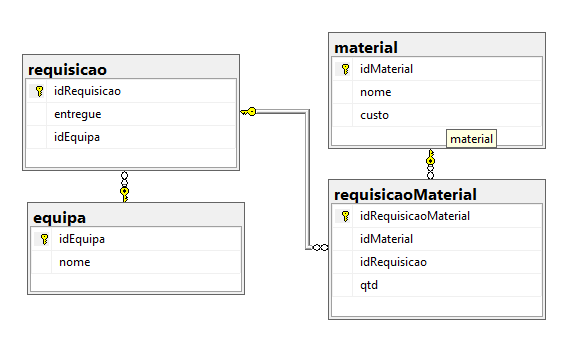
\includegraphics[scale=0.75]{imagens/basedadosRest.png}


\section{Serviço SOAP}

O registo de casos de novos casos CoViD assim como os respetivos contactos envolvem um ou vários utentes. Para tal é criada uma tabela Utente com chave primária idutente simbolizadora de um valor representativo de um cidadão como o NIF (ou até o Número de Cidadão) e ainda um nome.

A adição de um caso requer uma data de (deteção da infeção) e o id do utente a que este se refere. Cada caso tem o seu id individual e auto incrementado.

Caso este tenha entrado em contacto com outros cidadãos, os respetivos devem ser adicionados como membros da tabela Contactos, que estabelece relação entre o caso atribuído ao primeiro infetado e os cidadãos que estejam em risco de infeção. 

\vfill
\section{Importação de Ficheiros XML \& JSON}

A fiscalização do cumprimento das normas de isolamento envolve os utentes que são alvo da visita assim como irregularidades que possam ser encontradas durante esta última.

Para armazenamento destes dados adiciona-se as tabelas fiscalização e irregularidades, reutilizando a tabela já existente para o registo de casos no ponto anterior.

A tabela fiscalização mantém uma data de visita e o id do cidadão visitado.
Tendo em conta a possibilidade de deteção de várias irregularidades numa visita esta tabela mantém uma relação de um para muitos, guardando o id da fiscalização em causa e uma breve descrição da irregularidade detetada.